\documentclass{report}
\usepackage{graphicx} % Required for inserting images
\usepackage[italian]{babel}
\usepackage{tikz}
\usepackage{hyperref}
\usepackage{amsmath}
\usepackage{xcolor}

\definecolor{darkgreen}{rgb}{0.0, 0.5, 0.0}


\title{Preferenze privacy degli utenti}
\date{Parte IV}

\begin{document}

\maketitle

\tableofcontents
\newpage

\chapter{Introduzione}
\subsubsection{Privacy dell'identità degli utenti}
Gli utenti preferiscono restare anonimi o comunque non condividere troppe informazioni quando
operano nel cloud.
Alcune situe:
\begin{itemize}
    \item \textbf{Tecniche di comunicazione anonima}
    \item \textbf{Privacy in location-based services} (protezione della location quando sensibile)
    \item \textbf{Attribute-based control access:} è un problema lato server, non ci si basa più su chi un tente sia (l'identità)
        ma sugli attributi che ha (certificati che l'utente presenta)
    \item \textbf{Supporto alle preferenze privacy degli utenti} (problema lato utente)
\end{itemize}

Gli utenti potrebbero voler specificare le proprie scelte in termini di politiche del trattamento dei dati
\begin{itemize}
    \item l'utente decide quali informazioni inserire quando utilizza server esterni (es. Facebook)
    \item quando vengono rilascite informazioni nelle interazioni digitali (controllo dle rilascio dei dati)
\end{itemize}

due aspetti della protezione:
\begin{itemize}
    \item \textbf{rilascio diretto:} regola quando e perchè un utente rilascia informazioni (es. sto comprando qualcosa)
    \item \textbf{uso secondario:} regola l'uso e la profilazione dei dati da terze parti
\end{itemize}

\section{Rilascio diretto}
Definizione di meccanismi di \textbf{attribute-based access control} quindi di dipedenza dell'accesso rispetto alle proprietà che un utente ha.
Quello che gli utenti possono fare dipende dagli attributi che possiedono, verificati dai \textbf{certificati}

L'access control non risponde più si o no, ma risponde con i requisiti che il richiedente deve soddisfare per avere l'accesso.
Non solo i server vanno protetti ma anche gli utenti, per questo vanno introdotte \textit{forme di negoziazione}

Varie proposte tra cui:
\begin{itemize}
    \item credential/attribute policy specifications
    \item policy evaluation con informazioni parziali
    \item policy confidentiality support (anche la politica stessa potrebbe essere confidenziale)
    \item policy communication and dialog (come comunichiamo la politica)
    \item strategie di negoziazione e trust management (richieste e dimostrazioni continue dalle due parti)
    \item valutazione di terminazione, correttezza, nessuna informzione impropria nella negoziazione
\end{itemize}
tipicamente vengono usati linguaggi basati sul paradigma logico

\section{Controllo di acesso interattivo}
\begin{figure}[ht]
    \centering
    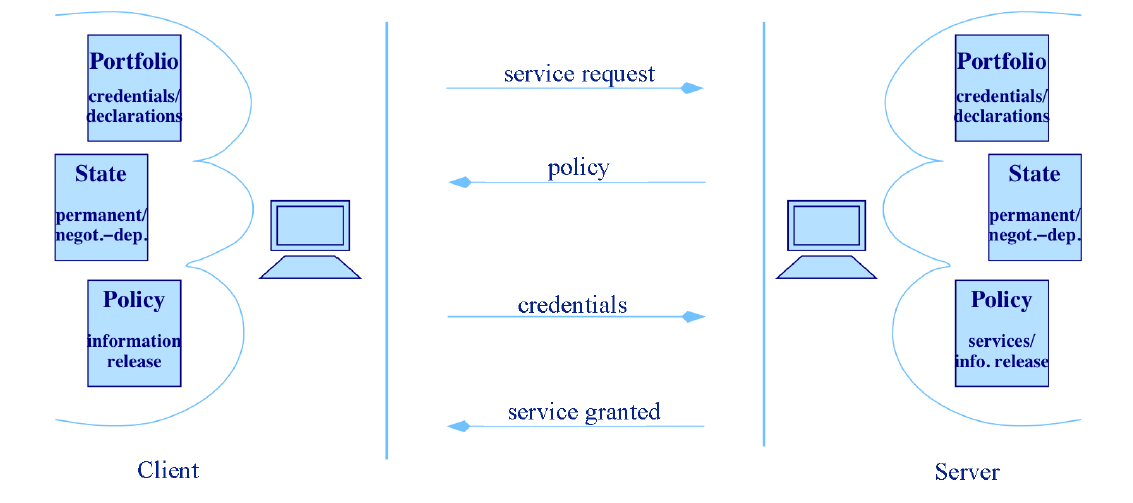
\includegraphics[width=1\linewidth]{images/interactive access control 1.png}
\end{figure}

Il client è colui che richiede il servzio, ha con se il suo \textbf{portoflio} (credenziali e proprietà), lo \textbf{stato}
(stato di informazioni che vuole mantenere) la \textbf{politica}, lo stesso vale per i server che è colui che offre il servizio.
La policy del server sta ad indicare ciò che il client deve dimstrare, tramite i certificati, per poter accedere al servzio.

\noindent Negozziazione multi-step implica \textit{Trust management} $ \rightarrow $ stabilire fiducia tra le due parti.

\begin{figure}[ht]
    \centering
    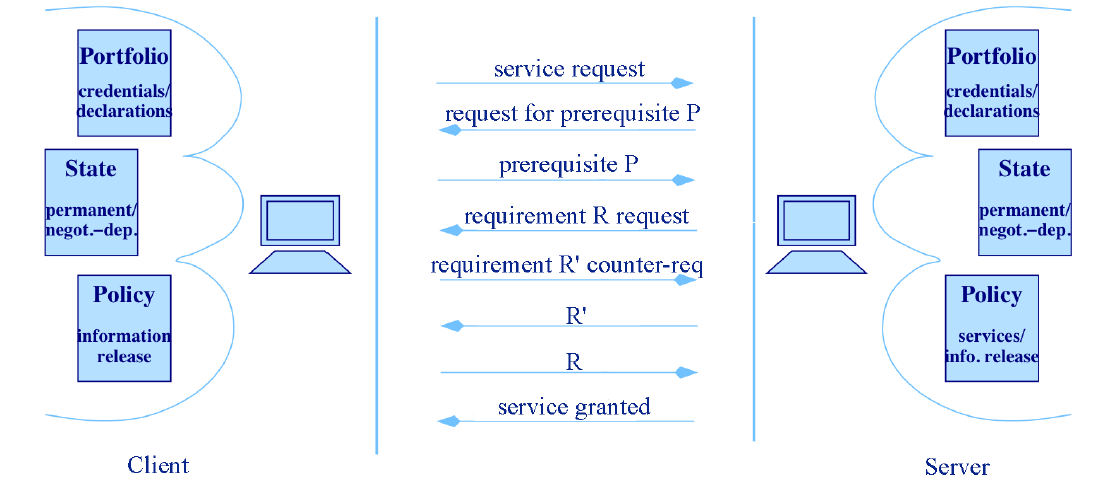
\includegraphics[width=1\linewidth]{images/interactive access control 2.png}
\end{figure}

\subsubsection{Interazione a due step:}
per essere gentili con l'utente separiamo i prerequsiti per l'accesso (necessari ma non sufficenti) e il requisito vero e proprio
con eventuale controrichiesta da parte dell'utente.

\subsubsection{Esistenti/emegenti tecnologie di supporto a ABAC}
\begin{itemize}
    \item U-Prove/Idemix: fornisce avanzate tecnologie di gestione dei certificati (i certificati odierni ti permettono di estrapolare dal certificato
    l'informazione senza fornire tutto il certificato).
    \item XACML: standard di oggi per l'interoperabilità delle politiche di controllo degi accessi
\end{itemize}

Le specifiche di controllo degli accessi non sempre fittano bene con il problema lato utente:
Di positivo hanno che sono espressive,potenti e permettono all'utente di di specificare se determinate informazioni possono o non possono essere rilasciate.
Di contro non permettono agli uenti di esprimere che preferirebbero rilasciare determinate informazioni piuttosto che altre, nel contesto in cui ne sia data la possibilità.

\begin{itemize}
    \item \textbf{Context-based preferences} (lascio la carta solo quando devo pagare)
    \item \textbf{Forbidden disclosures} (non vogliono che diverse personalità social siano linkate)
    \item \textbf{Associazioi sensibili}
    \item \textbf{Limited disclosure} 
    \item \textbf{Instance-based preferences}
    \item \textbf{History-based peferences} (magari ho già rilasciato qualcosa in passato)
    \item \textbf{Proof-based preferences}
    \item \textbf{Non-linkability preferences}
\end{itemize}
\end{document}